\section{Modello teorico}
\label{c:integr:model}

Prima di cominciare lo sviluppo, è di vitale importanza pensare al modello di integrazione della blockchain nel sistema, rappresentato in figura \ref{f:integr:modello}. 

%% METTERE IMMAGINE DEL MODELLO FINALE
% per l'immagine si fa una nuvoletta che rappresenta la siot, con dei cerchi che rappresentano i Server. i final client si connettono ai Server e le piattaforme 

Verrà creata un'applicazione che sarà utilizzata dall'utente finale per comprare i dati dei nodi della rete. 
Ognuna di esse è in grado di effettuare le transazioni, che saranno poi incluse nella blockchain. Ogni utente, attraverso l'applicazione, si connette con un nodo Server del GRIDS System. Quest'ultimo è incaricato di prendere i dati delle SVE che ospita (il Server stesso o gli altri Server della rete SIoT), attraverso i meccanismi di discovery descritti nel capitolo \ref{c:grids}, e di restituire i risultati all'utente finale. 

I proprietari dei nodi virtualizzati ed esposti attraverso la rete SIoT riceveranno il denaro virtuale, ma il GRIDS System terrà per sè una piccola percentuale del prezzo presentato all'utente finale.

I dati che verranno scambiati sono: l'utente fornisce ID del nodo a cui è interessato, il server risponderà con il prezzo dei dati corrispondenti. L'utente, venuto a conoscenza del prezzo, effettuerà la transazione e riceverà in cambio i dati del nodo IoT, oppure, nel caso si tratti di un nodo che appartiene a un canale Thingspeak, la readAPIkey con la quale l'utente potrà andare a leggere i dati autonomamente attraverso la piattaforma.

In sostanza, non vengono acquistati i dati direttamente dal sensore, ma viene aggiunto un livello di indirezione tra utente e nodo IoT, mantenendo il sistema ugualmente distribuito e decentrato, grazie all'utilizzo della blockchain.

I casi d'uso con cui verrà effettuato il testing riguarderanno un nodo Server del GRIDS System e un Client, ma sarà possibile utilizzare il sistema con una rete di Server e con Client multipli.

Sarà sviluppato, inoltre, un meccanismo di "ricarica" che permetterà al sistema di aggirare i tempi di conferma delle transazioni, che come sappiamo sono una caratteristica imprescindibile di qualsiasi blockchain, con il quale i client potranno effettuare un'unica transazione più grande e successivamente attingere dal credito residuo ogni qual volta desiderano acquisire dati dal sistema.

\section{Scelta della Blockchain}
\label{c:integr:lib}

La prima cosa da considerare per lo sviluppo del sistema è in modo in cui la blockchain può essere integrata. Sono possibili due principali modalità:
\begin{itemize}
    \item implementazione \textit{from scratch};
    \item utilizzo di una blockchain esistente.
\end{itemize}

L'implementazione \textit{from scratch} è una scelta poco pratica poiché è molto difficile reperire le risorse necessarie per il deployment di una blockchain, come ad esempio un numero considerevole di calcolatori per formare la rete di miners, e potenza computazionale sufficiente per l'esecuzione di un algoritmo per il raggiungimento del consenso.

Quindi la scelta naturale è l'uso di una blockchain preesistente attraverso \textit{reference implementation} o librerie. Nello specifico, è stata scelta la rete Bitcoin, con una community molto estesa di developer e un set di tool per potervi interagire, tra cui Bitcoinj\footnote{https://bitcoinj.github.io/}, una libreria implementata in Java, stesso linguaggio di programmazione utilizzato per lo sviluppo del GRIDS System. Le caratteristiche di questa libreria sono illustrate nel paragrafo \ref{c:integr:lib:bitcoinj}.
Un'altra feature della rete Bitcoin che ha influito positivamente sulla scelta della blockchain è la presenza di una Testnet, cioè una rete separata da Bitcoin Core in cui le transazioni non hanno alcun valore monetario. Essa è approfondita nel paragrafo \ref{c:integr:lib:testnet}.


\subsection{Bitcoinj}
\label{c:integr:lib:bitcoinj}

Bitcoinj è una libreria per lavorare con il protocollo Bitcoin. Può mantenere un wallet, inviare/ricevere transazioni senza aver bisogno di una copia locale di Bitcoin Core e ha molte altre caratteristiche avanzate. È implementata in Java, ma può essere utilizzato da qualunque linguaggio di programmazione JVM-compatible (come JavaScript).

Una caratteristica peculiare di Bitcoinj è la presenza della \textit{Simplified Payment Verification} (SPV): in questa modalità viene scaricata solo una piccola parte della blockchain, quindi è possibile utilizzare la libreria in dispositivi constrained, come i nodi dell'IoT. 

Altre caratteristiche di Bitcoinj sono: 
\begin{itemize}
    \item una \textit{wallet class} con cifratura, calcolo delle \textit{fees} (commissioni), derivazione deterministica della chiave e event listener che permettono di tenere aggiornato il saldo del wallet;
    \item un'applicazione con GUI per il wallet da utilizzare come base per le proprie app;
    \item \textit{full verification mode} sperimentale, che svolge lo stesso processo di verifica di Bitcoin Core. In questa modalità, il set di \textit{unspent transaction output} (UTXO set) viene calcolato e indicizzato in un database, permettendo un lookup veloce del saldo del wallet;
\end{itemize}

Ora andiamo ad approfondire il modello di sicurezza di Bitcoinj. Come gi\`a detto, questa libreria supporta due modalità: \textit{full verification} e \textit{simplified verification}. Esse controllano l'uso delle risorse dell'applicazione e quanta fiducia viene riposta negli altri partecipanti nel sistema Bitcoin. 

Come illustrato nel paragrafo \ref{c:tec:blockchain:funzionamento}, un nodo full mantiene un database di unspent outputs, e le transazioni che cercano di spendere output che non esistono oppure sono già stati spesi vengono ignorate. I blocchi vengono risolti dai miners e vengono inviati in broadcast nella rete cosicché tutti possano essere d'accordo sull'ordine delle transazioni e nodi che non vedono il broadcast di una certa transazione (per esempio perché erano offline in quel momento) possano recuperarla. 
Le operazioni di controllo, store e aggiornamento del database per ogni singola transazione è molto intenso; anche recuperare lo stato corrente del database from scratch è un'operazione molto lenta. Per questa ragione, non tutti i dispositivi possono mantenere un full node.

Con la SPV, invece, vengono memorizzate solo le transazioni rilevanti per il wallet in questione, mentre le altre vengono cancellate o direttamente mai scaricate. Le transazioni broadcast vengono sempre ricevute, però non ne viene controllata la validità. Questa modalità operativa è veloce e leggera abbastanza da essere eseguita su uno smartphone, ma può essere soggetta ad attacchi potenziali, illustrati qui di seguito: 

\begin{enumerate}
    \item \textit{Sybil attack}: consiste nel dirottare l'intera connessione internet della vittima e connetterla a una rete farlocca. È più facile da portare a termine quando viene utilizzata una connessione internet untrusted, come ad esempio reti Wi-Fi pubbliche, oppure utilizzando Tor. Bitcoinj non supporta Tor, quindi gli interessati da questo attacco possono essere i wallet mobili; 
    \item \textit{Finney attack}: consiste nel risolvere un blocco che contiene un double spend, comprare un servizio, e poi inviare in broadcast il blocco.
\end{enumerate}

Per spiegare meglio il funzionamento di questi attacchi, bisogna prima introdurre il concetto di \textit{pending transaction}.

Una \textit{pending transaction} è una transazione non ancora inclusa nella blockchain; in altre parole, è lo stato che assume non appena viene diffusa nella rete. I nodi miners che vedono questa transazione, ne controllano la validità e, se il risultato è positivo, la includono nel blocco che al momento stanno provando a risolvere. Naturalmente, quelle non valide vengono ignorate.

L'applicazione del client riceverà le \textit{pending transactions}, le aggiungerà al wallet e avvierà gli event listener. Tuttavia, nella modalità SPV l'unico motivo che si ha per credere che la transazione sia valida è il fatto che i nodi a cui si è connessi trasmettano la transazione nella rete. Se un'applicazione fosse connessa a un nodo malevolo, quest'ultimo potrebbe passare all'applicazione delle transazioni completamente invalide (come \textit{double spend} o addirittura transazioni con soldi inesistenti), e verrebbero ugualmente prese per buone. 

Dato che le applicazioni sviluppate con Bitcoinj non accettano connessioni in entrata, i peer con cui esse comunicano sono sempre scelti in maniera casuale all'avvio, quindi diventa estremamente difficile per un aggressore controllarne la connettività. Per questa ragione, il numero di peer che hanno confermato una transazione viene esposto attraverso l'oggetto \textit{TransactionConfidence}, e l'applicazione è in grado di monitorarlo per avere questo tipo di informazione. Questa feature, come verrà spiegato più avanti, sarà molto utile per lo sviluppo dei wallet del GRIDS System.

Una volta che la maggior parte dei peer hanno confermato quella transazione, si può essere abbastanza sicuri che essa si sta propagando attraverso la rete e con ogni probabilità è valida: ecco il motivo principale per cui il Sybil attack è molto improbabile.

In un Finney attack, invece, l'attaccante crea un blocco che include una transazione tra due indirizzi controllati da lui. Una volta estratto il blocco, non lo diffonde subito, ma invece va a spendere quella valuta da qualche venditore che accetta transazioni non confermate. Una volta ottenuti i beni dal venditore, diffonde il blocco contenente il double spend, e quindi riceve i soldi indietro. Tutto questo processo richiede una buona dose di tempismo e pazienza da parte dell'attaccante: non solo deve risolvere correttamente il blocco, ma deve anche effettuare velocemente l'acquisto del bene, prima che un altro miner riesca a risolvere e a diffondere un altro blocco valido. In conclusione, un utente che vende beni in maniera irreversibile, in maniera veloce e che accetta transazioni non confermate è suscettibile a un attacco Finney.

Questo problema viene risolto da parte di Bitcoinj attraverso l'utilizzo della \textit{Transaction Confidence}: se qualcuno perpetra un attacco, la confidence per quella transazione assumerà il valore \textit{DEAD}, il che significa che la transazione è come invertita e non verrà considerata per il conteggio del wallet della vittima.
La \textit{transaction confidence} è lo strumento di forza di Bitcoinj: permette di sapere se una certa transazione è inclusa o meno nella blockchain. 
Quando una transazione viene aggiunta nella blockchain, la transaction confidence assume il valore \textit{BUILDING} e si può accedere alla \textit{transaction depth}, ossia il numero di blocchi che sono stati costruiti a partire dal blocco della transazione stessa (per esempio, una transazione appena confermata ha depth uguale a 1).
Inoltre, sono implementati degli event listener che, ascoltando gli eventi della rete, possono essere usati per scatenare azioni specifiche nell'applicazione utente, come spedire beni o servizi soltanto quando viene raggiunto un certo livello di confidence.

Nel caso del nostro sistema, i listener che monitorano la confidence delle transazioni serviranno per innescare lo scambio di dati tra i client e la piattaforma SIoT.

%%%%%%%%%%%%%%%%%%%%%%%%%%

\subsection{Testnet}
\label{c:integr:lib:testnet}

La Testnet è un'alternativa alla blockchain della rete Bitcoin ufficiale, per essere utilizzata a fini di testing. Le monete della Testnet sono separate e distinte dai bitcoin reali e non hanno alcun valore. Ciò permette agli sviluppatori di applicazioni bitcoin-based di evitare di utilizzare veri bitcoin, senza la preoccupazione di perderli o di rompere la blockchain principale.

Per utilizzare la Testnet invece della rete principale, basta inserire un flag nell'applicazione: nel caso specifico di Bitcoinj, bisogna selezionare i \textit{Network Parameters} relativi alla Testnet.

La testnet è attualmente alla terza versione. La prima era stata superata poiché aveva il grosso problema secondo cui gli utenti cominciavano a scambiare la valuta della testnet con bitcoin reali, quindi è stata introdotta la versione 2, superata ulteriormente dalla versione attuale, che verifica le transazioni in minor tempo e contiene all'interno della propria blockchain transazioni \textit{edge-case} che ne testano la compatibilità implementativa.

Le differenze con la rete Bitcoin ufficiale sono:
\begin{itemize}
    \item il protocollo di rete della testnet utilizza la porta 8333 invece che la 18333 della rete Bitcoin;
    \item i valori nel campo ADDRESSVERSION sono differenti, per assicurare che nessun indirizzo della testnet funzioni nella rete Bitcoin;
    \item vi sono diversi header nel messaggio del protocollo: 0x0B110907 della rete ufficiale contro 0xF9BEB4D9 della testnet;
    \item la difficoltà minima di 1.0 nella testnet è uguale alla difficoltà 0.5 della rete principale. Ciò significa che la difficoltà della testnet è doppia rispetto a quella della rete Bitcoin. Inoltre, se nessun blocco viene risolto entro 20 minuti, la difficoltà viene resettata al valore minimo;
    \item un genesis block diverso;
    \item nella testnet è possibile utilizzare transazioni non-standard.
    \item la testnet riceve meno transazioni rispetto la blockchain principale ed è solitamente più piccola in termini di GB.
\end{itemize}

Per acquisire bitcoin utili per operare nella testnet, si possono utilizzare delle \textit{faucet} dalle quali è possibile ricevere valuta di testing\footnote{https://testnet.manu.backend.hamburg/faucet}. È buona norma, dopo averli utilizzati, ridare indietro i bitcoin alla faucet.

\section{Interfaccia Web e REST}
\label{c:integr:webrest}

È stata costruita un'interfaccia web con Angular 2 che interagisce con l'interfaccia REST del sistema, per rendere più agevole l'interazione con il sistema. In figura \ref{f:integr:gui-web} è rappresentata la GUI.

\begin{figure}[h!t]
\centerline{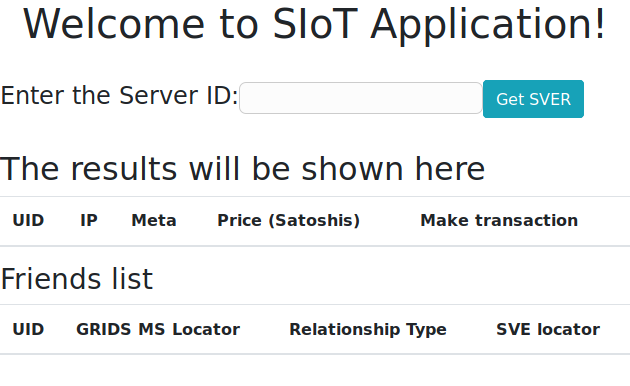
\includegraphics[scale=2.5]{img/gui-web-app}}
\caption{Interfaccia grafica della web app}
\label{f:integr:gui-web}
\end{figure}

Per quanto riguarda le REST API, invece, è stata aggiunta nella risorsa REST "Server" (a fini di testing) una richiesta che effettua una transazione da parte del server SIoT verso il wallet del proprietario del nodo IoT per ottenere alcuni dati, per esempio l'elenco delle relazioni del nodo.
\begin{itemize}
    \item Metodo: GET
    \item Path: "{id}/SVER/{uid}/Transaction/{amount}/{address}"
\end{itemize}

I parametri \textit{id} e \textit{uid} sono analoghi a quelli citati nel paragrafo \ref{c:grids:implementation}, mentre \textit{amount} e \textit{address} sono rispettivamente il numero di satoshi da inviare e l'indirizzo del wallet di destinazione.

È stata inoltre aggiunta la risorsa REST aggiuntiva "Transaction", di cui è riportato un estratto nel listing \ref{restResource}, che raccoglie le richieste per l'interazione con il Transaction Manager. È stata definita una richiesta che permette di visualizzare i dati ottenuti a seguito di una transazione.
\begin{itemize}
    \item Metodo: GET
    \item Path: "{trxHash}", dove trxHash è l'hash della transazione di cui si vuole visualizzare il risultato.
\end{itemize}

Nel caso d'uso considerato per lo sviluppo del sistema, con questa richiesta verrà restituita la \textit{Thingspeak readAPIkey} corrispondente al nodo di cui si desiderano i dati.


\begin{lstlisting}[caption={TransactionResource.java},label={restResource},style={c}]

@GET
@Path("{trxHash}")
@Produces(MediaType.TEXT_PLAIN)
public String visualizeData(@PathParam("trxHash") String trxHash) {
    // search the trx in the DB
    trxManager = new TrxManager();
    String result;
    if (trxManager.isUnconfirmed(trxHash)) {
        result = "Waiting for transaction validation...";
    } else {
        // get the data of transaction
        result = trxManager.getCompletedTrx(trxHash);
    }
    trxManager.closeConnection();
    return result;
}
\end{lstlisting}

\section{Database}
\label{c:integr:db}

Per quanto riguarda la parte di Data Access, è stato creato un nuovo database, oltre ai due preesistenti, chiamato \textit{social\_iot\_platform\_transaction}, in cui sono contenute quattro tabelle necessarie per l'implementazione delle transazioni.

La tabella "completed" contiene tutte le transazioni che sono state incluse nella Blockchain, insieme ai dati da restituire al Final Client. I campi sono i seguenti:

\begin{itemize}
    \item \textbf{TrxHash}: hash della transazione confermata;
	\item \textbf{content}: stringa con i dati.
\end{itemize}

La tabella "unconfirmed" contiene tutte le transazioni non ancora confermate. I campi sono:

\begin{itemize}
    \item \textbf{TrxHash}: hash della transazione da confermare;
    \item \textbf{SVER\_ID} e \textbf{SVE\_ID} del nodo di cui sono stati richiesti i dati.
\end{itemize}

La tabella "creditCharges" registra tutte le ricariche eseguite dagli utenti:

\begin{itemize}
    \item \textbf{trxHash}: hash della transazione confermata;
	\item \textbf{userID}: numero identificativo del Final Client. Al momento viene settato manualmente per ogni utente, ma successivamente potrebbe essere implementato un meccanismo di "log in" in cui sarà il GRIDS System a fornire dinamicamente un ID;
	\item \textbf{credit}: valore del credito ricaricato (in satoshi);
	\item \textbf{isConfirmed}: valore booleano che memorizza se la transazione è stata inclusa o meno nella Blockchain. Delle funzioni apposite del Transaction Client (paragrafo \ref{c:integr:trxmanager}) provvederanno a impostare il valore corretto di questo campo.
\end{itemize}

La tabella "readAPIkeys", infine, contiene, come dice il nome stesso, le readAPIkey di tutti i nodi ospitati dal GRIDS System. Essa verrà consultata 

\section{RMI registry}
\label{c:integr:rmi}

La Java API che permette di eseguire la \textit{remote method invocation} è l'elemento fondamentale della comunicazione tra le entità del sistema. Oltre all'interfaccia già esistente per l'interazione tra i Server del GRIDS System, è stata creata un'ulteriore interfaccia RMI per la comunicazione tra Server e Final Client: quest'ultima, però, è stata separata dalla prima per garantire il disaccoppiamento tra i metodi invocabili dai Server per la creazione dei propri wallet e i metodi per la richiesta di dati da parte dei Final Client. Perciò è presente un processo aggiuntivo in ascolto sulla porta 4849, diverso dal processo rmiregistry in ascolto sulla porta di default 1099, nella quale verrà effettuato il binding dei metodi della FinalClientRMIRootInterface, illustrata più avanti.

I metodi che sono stati aggiunti all'interfaccia RMI già esistente sono i seguenti:

\begin{itemize}
    \item CreateWallet(): permette la creazione del wallet destinato al nodo Server;
    \item getWalletBalance(): restituisce la quantità di valuta presente all'interno del wallet;
    \item makeTransaction(String destAddress, String amount): permette di effettuare una transazione di una quantità \textit{amount} di bitcoin all'indirizzo \textit{destAddress}.
\end{itemize}

I metodi dell'interfaccia FinalClientRMIRoot, riportati nel listing \ref{FinalClientRMIRootInterface}, vengono implementati all'interno del Server, e sono accessibili dai Final Client. Essi sono:

\begin{itemize}
    \item requestDataWithTrx(): aggiunge la transazione nella lista di quelle non confermate e restituisce l'indirizzo web in cui verranno visualizzati i risultati una volta che la transazione sarà validata;
    \item rechargeCredit(): ricarica il credito dell'utente con \textit{userID};
    \item getCredit(): restituisce il valore del credito residuo (in satoshi) dell'utente con \textit{userID};
    \item requestDatawithCredit(): permette di effettuare la richiesta dei dati 
\end{itemize}

\begin{lstlisting}[caption={FinalClientRMIRootInterface.java},label={FinalClientRMIRootInterface},style={c}]

public interface FinalClientRMIRootInterface extends Remote {
    
    public String requestDataWithTrx(String txHash, String SVER_ID, String SVE_ID) throws RemoteException;
    
    public String rechargeCredit(String trxHash, int userID, int amount) throws RemoteException;
    
    public int getCredit(int userID) throws RemoteException;
    
    public String requestDatawithCredit(String SVER_ID, String SVE_ID, int userID) throws RemoteException;
}

\end{lstlisting}

Nell'implementazione dei metodi appena elencati vengono istanziati oggetti di una classe chiamata \textit{Transaction Manager}, il punto focale del meccanismo di esecuzione e verifica delle transazioni, ma anche dell'accesso ai dati. Nel paragrafo \ref{c:integr:trxmanager} sarà illustrato nel dettaglio.

\section{Wallet Bitcoin e Transaction Manager ?}
\label{c:integr:trxmanager}


Il wallet Bitcoin, prima di essere integrato all'interno del GRIDS System, è stato sviluppato separatamente, come mostrato nel diagramma \ref{f:integr:trxclient}, ??per esigenze di testing??. L'interfaccia \textit{TransactionIf} contiene le \textit{signature} delle funzioni basilari per il funzionamento del wallet, come ad esempio makeTransaction(). La classe \textit{TransactionClient} contiene le implementazioni di tali metodi e gli attributi kit e params, rispettivamente delle classi \textit{WalletAppKit} e \textit{NetworkParameters} della libreria Bitcoinj. Nel listing \ref{trxClient} viene riportata l'implementazione del metodo makeTransaction(). Nel corpo del codice si può osservare l'istanziazione di una SendRequest che specifica, oltre all'oggetto Address contenente l'indirizzo del wallet destinatario, la quantità di valuta da scambiare. Viene poi aggiunta una commissione (in questo caso è la \textit{minimum fee} di riferimento della rete Bitcoin) e, cosa più importante, viene verificato che il risultato della richiesta non sia nullo, per evitare di generare una transazione che spendi più soldi di quanti non ne abbia il wallet del mittente. CheckNotNull() è una funzione di \textit{Guava} (Google core libraries for Java).

%listing trx client
\begin{lstlisting}[caption={Metodo makeTransaction in TransactionClient.java},label={trxClient},style={c}]

public Transaction makeTransaction(String destAddress, String amount) 
{
Transaction transaction = null;
System.out.println("Sending " + amount + " satoshis to " + destAddress);
Address address = Address.fromBase58(this.params, destAddress);
try {
    SendRequest sendRequest = SendRequest.to(address,
            Coin.valueOf(Long.parseLong(amount)));
    sendRequest.feePerKb = Transaction.REFERENCE_DEFAULT_MIN_TX_FEE;
    Wallet.SendResult sendResult = this.getWallet().sendCoins(
            this.getKit().peerGroup(), sendRequest);
    checkNotNull(sendResult); 
    transaction = sendResult.broadcastComplete.get();
    System.out.println("coins sent. transaction hash: "
            + transaction.getHashAsString());
} catch (InsufficientMoneyException e) {
    System.out.println("Not enough coins in your wallet. Missing "
            + e.missing.getValue() + " satoshis are missing (including fees)");
} catch (InterruptedException | ExecutionException ex) {
    Logger.getLogger(TransactionClient.class.getName()).log(Level.SEVERE, null, ex);
}
return transaction;

}
\end{lstlisting}

\begin{figure}[h!t]
\centerline{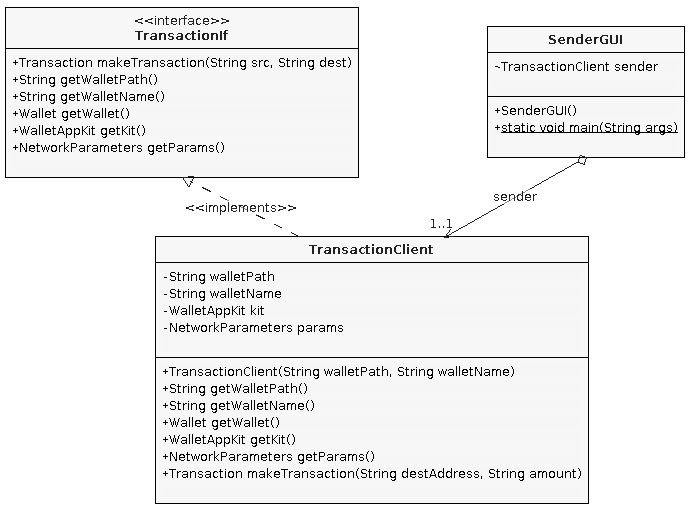
\includegraphics[scale=2]{img/BlockchainCorrect}}
\caption{Diagramma delle classi del Transaction Client}
\label{f:integr:trxclient}
\end{figure}

Il \textit{Transaction Manager} è lo strato software in cui vengono implementate tutte le funzioni di gestione del meccanismo di ricezione dei soldi e restituzione dei dati. 

Il Transaction Manager che si trova all'interno del nodo Server del GRIDS System è composto dalle seguenti classi Java:

\begin{itemize}
    \item TrxManager:
    \item SIoTBitcoinClient:
    \item WalletWrapper:
    \item TransactionResource:
\end{itemize}

Cascata di codice e diagrammi!

\section{Interfacce grafiche ???????}
\label{c:integr:gui}

Aggiungere screenshot della GUI


\section{Casi d'uso}
\label{c:integr:useCase}

Mettere l'acquisto lento, la ricarica, e l'acquisto veloce


ALTRO:

- dire del problema che bisogna aspettare la conferma delle trx di volta in volta, quindi si è pensato di velocizzare l'acquisto dei dati con metodo "a ricarica".

- mettere il sito https://testnet.blockchain.info/ in cui è possibile vedere tutti i blocchi della blockchain in tempo reale